\chapter{Evaluation}\label{chapEvaluation}

The previous chapters explained the algorithm and challenges which must be solved in order to find any solution. Thereby they did not focus on the execution time and the quality of the resulting software. In this chapter, the first goal is to identify a recommended configuration among the many possible. It has to create a solution in a reasonable time and with a reasonable probability. The second goal is to analyze the behavior of the algorithm in terms of convergence and the chance of getting trapped in a \gls{LocalOptimum} according to sub-section \ref{secEvolutionaryAlgorithms} and section \ref{secSelectionReplacementStrategies}. Finally, the third goal is the evaluation of the software quality of the created solutions. This is required, since a manual adaption is expected in some cases (see section \ref{secSolutionOverview}).

A rough overview of the evaluated configurations and the dimensions is presented at first in section \ref{secEvaluatedConfigurationsAndDimensions}. Afterwards, the recommended configuration is presented in section \ref{secRecommendedConfiguration}, followed by an analysis of the chosen settings compared to the others in section \ref{secConvergenceAndLocalOptimum}. The maintainability of the results is evaluated in section \ref{secMaintainabilityOfResults}.

\section{Evaluated Configurations and Dimensions}
\label{secEvaluatedConfigurationsAndDimensions}

\textbf{Evaluated Configurations}: All presented configuration options are part of the evaluation. The ones which are based on numerical data are evaluated with a few values starting with a low value. They end with a high value that is expected to be close to an unacceptable execution time.
\begin{itemize}
\item Scenarios
	\begin{enumerate}
	\item Simple
	\item Complex
	\end{enumerate}
%\item Mutations

\item Mutation Selection Strategies
	\begin{enumerate}
	\item Selection option from all possible (Option)
	\item Select operator first and then an option (Operator $\rightarrow$ Option)
	\end{enumerate}
	
\item Selection and Replacement Strategies
	\begin{enumerate}
	\item Naive approach with high selection pressure and elitism
	\item Roulette wheel selection with elitism
	\item Tournament selection with elitism - Tournament size of 10
	\item Tournament selection with elitism - Tournament size of 2
	\end{enumerate}
	
\item Fitness Function Configurations
	\begin{enumerate}
	\item Class focused using Name
	\item More class focused using Name
	\item Class focused using heuristic
	\item Class focused using Name and heuristic fall-back
	\item Class and association focused using name and heuristic fall-back
	\item Property focused using Name and heuristic fall-back
	\end{enumerate}	
	
\item Maximum Number of Generations: 50, 100, 200
%	\begin{enumerate}
%	\item 50
%	\item 100
%	\item 200
%	\end{enumerate}
\item Population Size: 10, 50, 100, 200
%	\begin{enumerate}
%	\item 10
%	\item 50
%	\item 100
%	\item 200
%	\end{enumerate}
\end{itemize}

These configuration options result in about 1.000 configurations which need to be analyzed. Since the execution of a configuration always includes randomness, each configuration is executed 50 times. Overall, this resulted in about 50.000 \glspl{Population} with 300.000.000 \glspl{Individual}, a total runtime of about 32 days and 27 gigabyte of data.

\textbf{Evaluated Dimensions}: In order to answer the previously mentioned questions about the quality of the configurations, the dimensions presented in the following are measured. The aggregations are evaluated based on all 50 executions of each configuration to reduce the impact of randomness.
\begin{itemize}
\item Number of Solutions: Sum, Minimum, Average, Maximum %Range: 0 - Population Size, Aggregations: Average
\item Runtime: Sum, Minimum, Average, Maximum %Range: 0s - infinite, Aggregations: Average
\item Fitness: Minimum, 25$^{th}$ Percentile, Median, 75$^{th}$ Percentile, Maximum per \gls{Generation} %Range: 0 - 100\%, Aggregations: Maximum, Minimum, Quartiles, Quantiles, Median
\end{itemize}
The first two are aggregated using the functions sum, minimum, average and maximum in order to determine the expected solutions and runtime and thereby answer the fundamental questions. Analyzing the termination and \gls{LocalOptimum} trap is the goal of the fitness-dimension. Therefore, the \gls{GeneticDiversity} has to be examined, which is performed by the fitness distribution analysis of each \gls{Population} per \gls{Generation}. Such distributions of values are visualized with box-and-whisker plots that are based on the minimum, 25$^{th}$ percentile, median, 75$^{th}$ percentile and maximum. Thus, those values are measured for each \gls{Generation} in order to be able to analyze the development of a \gls{Population}.


\section{Recommended Configuration}
\label{secRecommendedConfiguration}

The large amount of configurations renders an in depth comparison of all configurations impossible within this thesis. Hence, the analysis is based on a divide-and-conquer approach. Therefore, at first the results of the configurations are separated by the scenario. In the simple scenario all configurations except for 6\% found at least one solution. All of the failed configurations used a population of size ten, thus this size cannot be recommended. The measured runtime of a single execution of a successful configuration was on average three seconds and at least 17 seconds. This is an acceptable time even when considering 50 executions. In contrary, the complex scenario has not been solved in 84\%, while the same execution took on average 5 minutes and at least about 30 minutes. Since a single execution also does not always return a solution, the time of the 50 executions has to be considered which ranges from 45 minutes to 15 hours for the complex scenario. The used computer has an Intel Core i7 CPU with eight logical processors each working with 3.4 GHz, 32 GB RAM and a 250 GB SSD disk.

It hat to be pointed out that the implementation was not focused on performance, thus the execution times can probably be reduced a lot. Especially, the excessive reporting required at lot of computational power, though it is not required in an end-user environment. Nevertheless, a recommendation for the current prototype has to be presented, which returns a solution with a sufficient probability in an acceptable time. 

\begin{figure}[!ht]
	\centering
	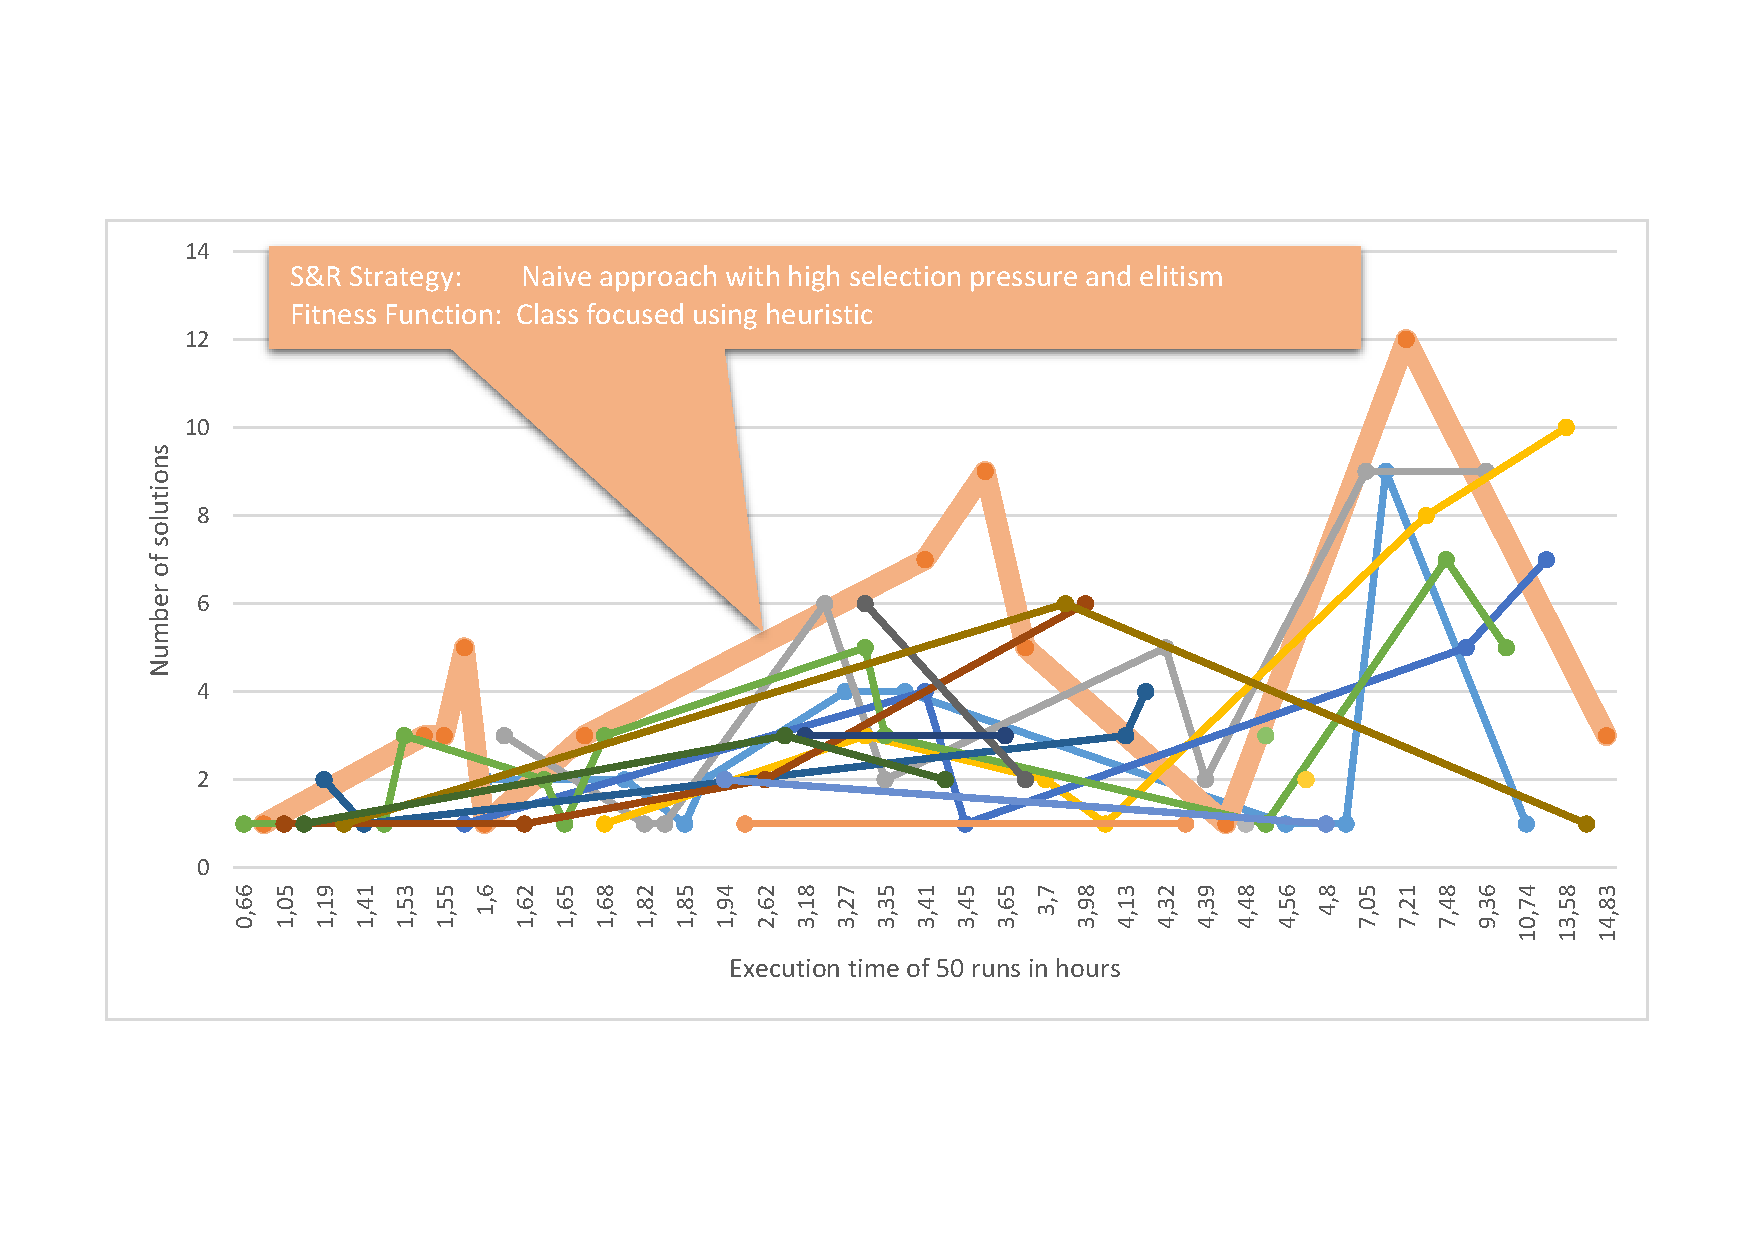
\includegraphics[scale=0.55, trim=1.5cm 3.5cm 1.5cm 3.5cm, clip=true]{Images/ConfigurationComparison3.pdf} 
	\caption{Configuration comparison for complex scenario - Each value is the result of the 50-time execution of a configuration. All configurations with the same Fitness Function as well as the same Selection and Replacement Strategy are equally colored and connected.}
	\label{figConfigurationComparison3}
\end{figure}

Hence, the configurations executed with the complex scenario are compared by the number of returned solutions and total execution time in figure \ref{figConfigurationComparison3}. The number of solutions ranges from 1 to 12, whereas the execution stops in the case a solution is found. Furthermore, a single \gls{Population} can contain as many solutions as it has \glspl{Individual}. In order to identify an ideal configuration within the large set, at first the population size, maximum number of generations and the Mutation Selection Strategy are excluded. It resulted in a connection of configurations with the same Selection and Replacement Strategy and Fitness Function. The ``Naive approach with high selection pressure and elitism" with the ``Class focused using heuristic" configuration outperforms the others in number of successful configurations, number of solutions and execution time of the 50 runs overall.

After two of five configuration settings are identified, the next step is to analyze the Mutation Selection Strategy. The maximum number of \glspl{Generation} and the \gls{Population} size are increasing the entropy, but are not changing the general behavior of the algorithm. Therefore, those two are the last to be analyzed.

\begin{figure}[!ht]
	\centering
	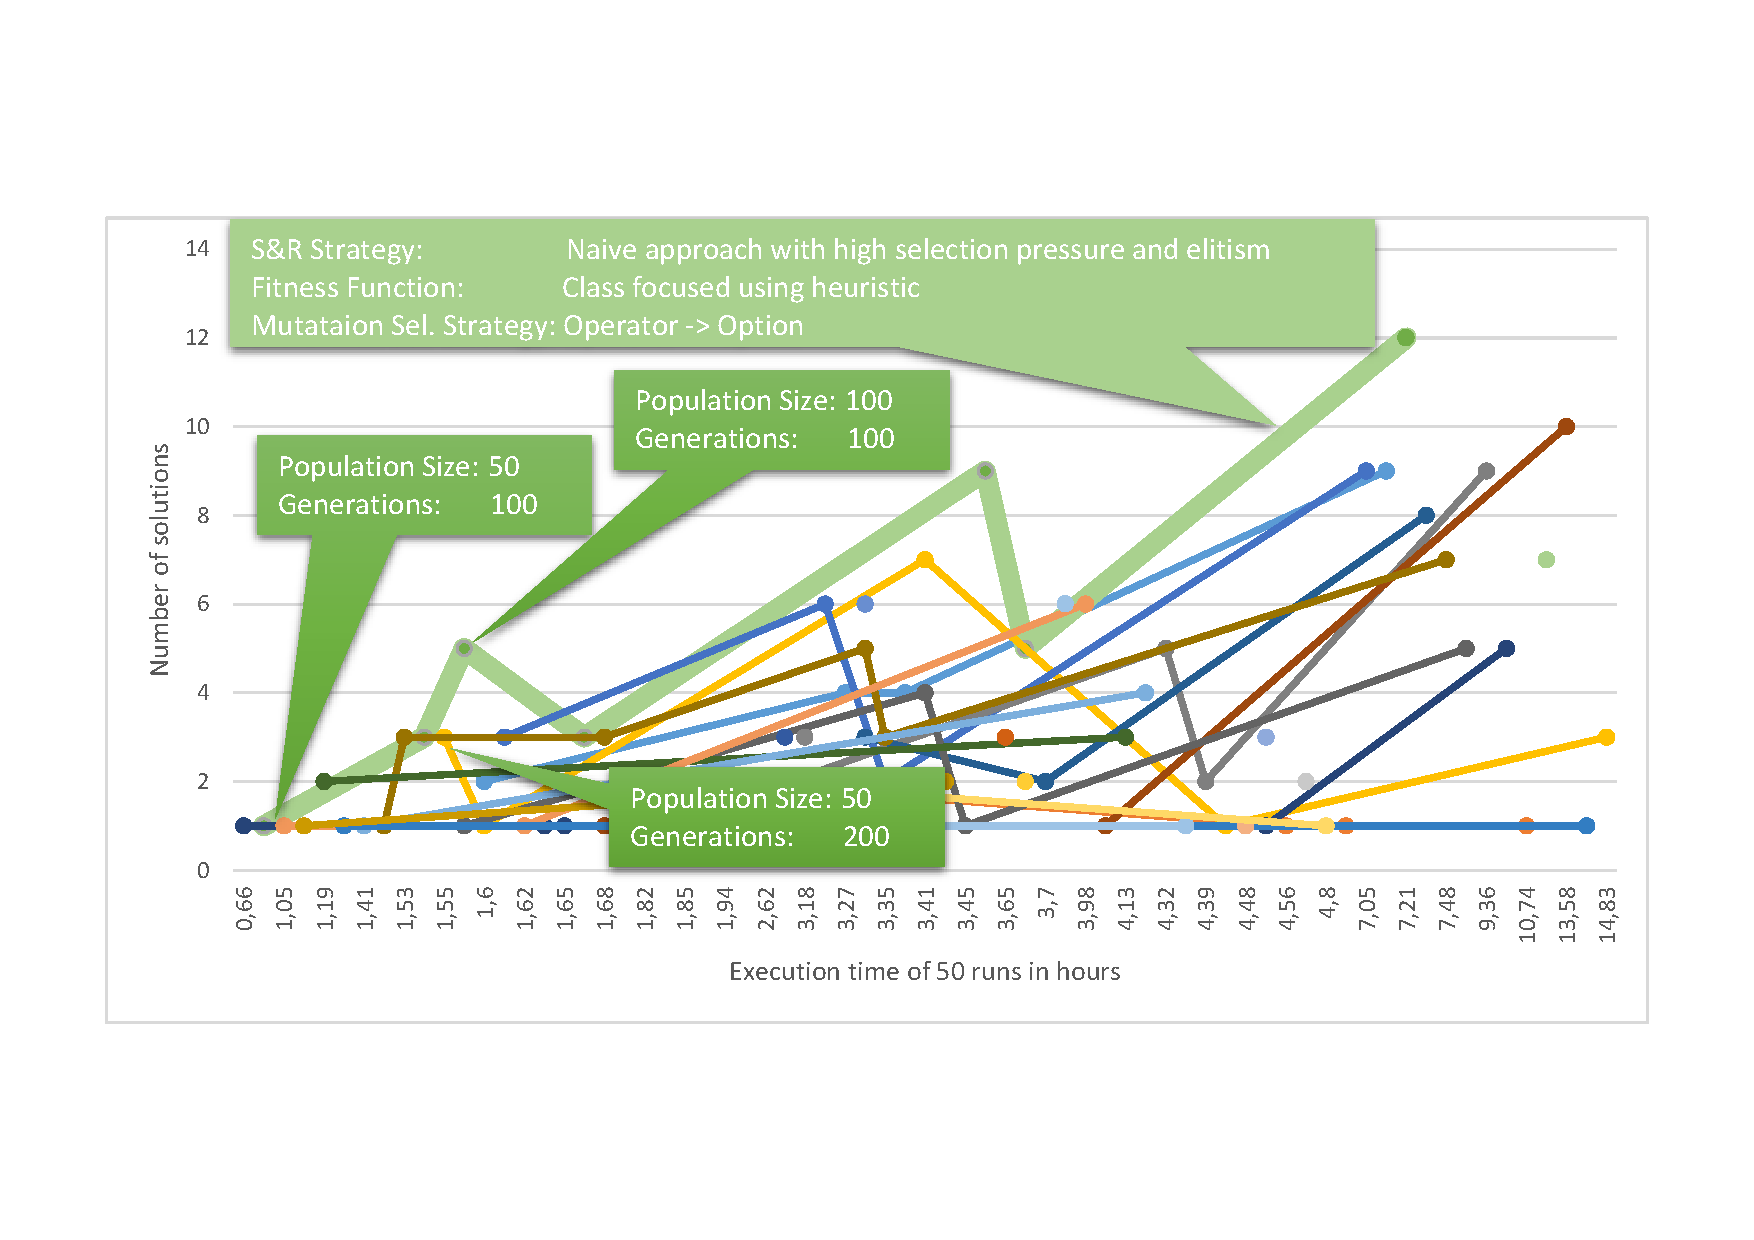
\includegraphics[scale=0.55, trim=1.5cm 3.5cm 1.5cm 3.5cm, clip=true]{Images/ConfigurationComparison2.pdf} 
	\caption{Configuration comparison for complex scenario - Each value is the result of the 50-time execution of a configuration. All configurations with the same Fitness Function, Selection and Replacement Strategy as well as Mutation Selection Strategy are equally colored and connected.} %, except for the population size and maximum number of generations, 
	\label{figConfigurationComparison2}
\end{figure}

Figure \ref{figConfigurationComparison2} adds the Mutation Selection Strategy to the settings used to connect the configurations. The ``Operator $\rightarrow$ Option"-Strategy thereby outperforms the others. In figure \ref{figConfigurationComparison2} the maximum number of \glspl{Generation} and \gls{Population} size of the first three configurations of this setting is shown. The first two have a \gls{Population} size of 50 using 100 resp. 200 \glspl{Generation} while returning only one resp. three solutions in 0.74 resp. 1.52 hours. However, the third one requires with 1.58 hours slightly more time, but returns five solutions.

Hence, a solution can be found in less than an hour. Since the number of solutions is subject to random effects, the more reliable to expect two hours. Within this recommended configuration the maximum number of \glspl{Generation} is 100 and also the \gls{Population} size is 100. An increasing number of \glspl{Generation} and / or a increased \gls{Population} size can be used to extend the entropy. Thereby the chance to find a solution with more computational power and / or in a larger timespan is increased.



\section{Convergence and Local Optima} %Termination
\label{secConvergenceAndLocalOptimum}

After presenting a recommended configuration, this section focuses on the analysis of the \gls{GeneticDiversity} based on the fitness development. In particular, the goal is to analyze why the chosen settings outperformed the others and if the recommended setting is hazard to become trapped in a \gls{LocalOptimum}. Again, in this section the simple scenario is not analyzed, since almost all configurations succeeded in an acceptable time whereas the complex scenario shows the opposite behavior.

\begin{figure}[!ht]
	\centering
	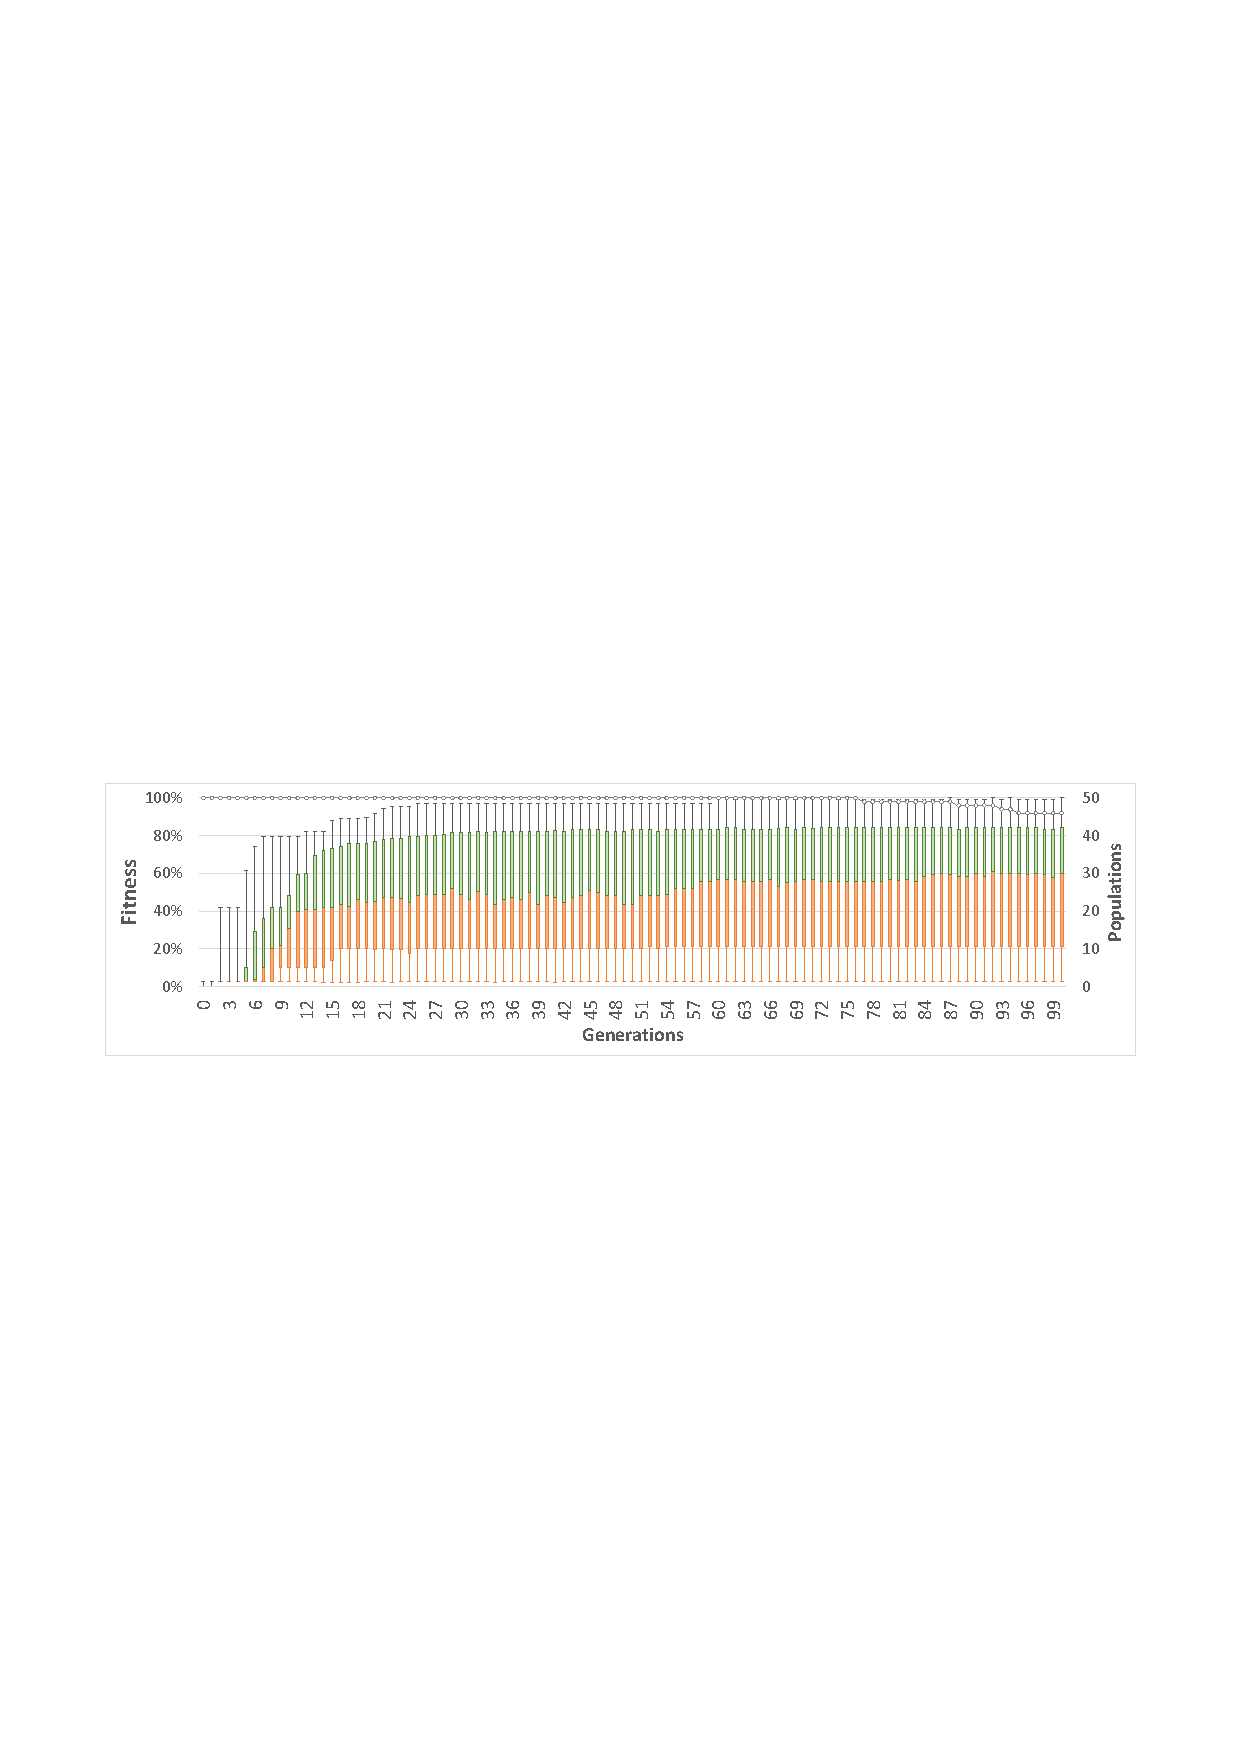
\includegraphics[scale=0.8, trim=1.5cm 11.5cm 1.5cm 13cm, clip=true]{Images/ConfigurationComparison_BestWithOperatorOption.pdf} 
	\caption{Fitness development of recommended configuration. The box-and-whisker plot shows the fitness of the 50 \glspl{Population} per \gls{Generation} on the primary axis. The secondary axis states the number of \glspl{Population} which did not yet return a solution and hence are further evaluated.}
	\label{figConfigurationComparison_BestWithOperatorOption}
\end{figure}

Figure \ref{figConfigurationComparison_BestWithOperatorOption} shows the fitness development per \gls{Generation} in a box-and-whisker plot using the recommended configuration. A general observation is that the maximum fitness increases steadily and that the fitness distribution is balanced. Hence, the recommended solution is expected be robust and will not very likely become stuck in a \gls{LocalOptimum}.

% analyse native and heuristc (best) configuration
% erklären warum sr und ff so gut sind 
% especially the s&p strategies that should avoid local optima converged often too slowly
% example of tournament 10 and naive (see previous figure) (size 2 and roulette performed better, but below naive)

\textbf{Selection and Replacement Strategy analysis}: Comparing the recommended setting to the ``Tournament selection with elitism - Tournament size of 10"-Selection and Replacement Strategy, shows that this strategy is inertial. Even though the fitness distribution becomes balanced in later \glspl{Generation}.

\begin{figure}[!ht]
	\centering
	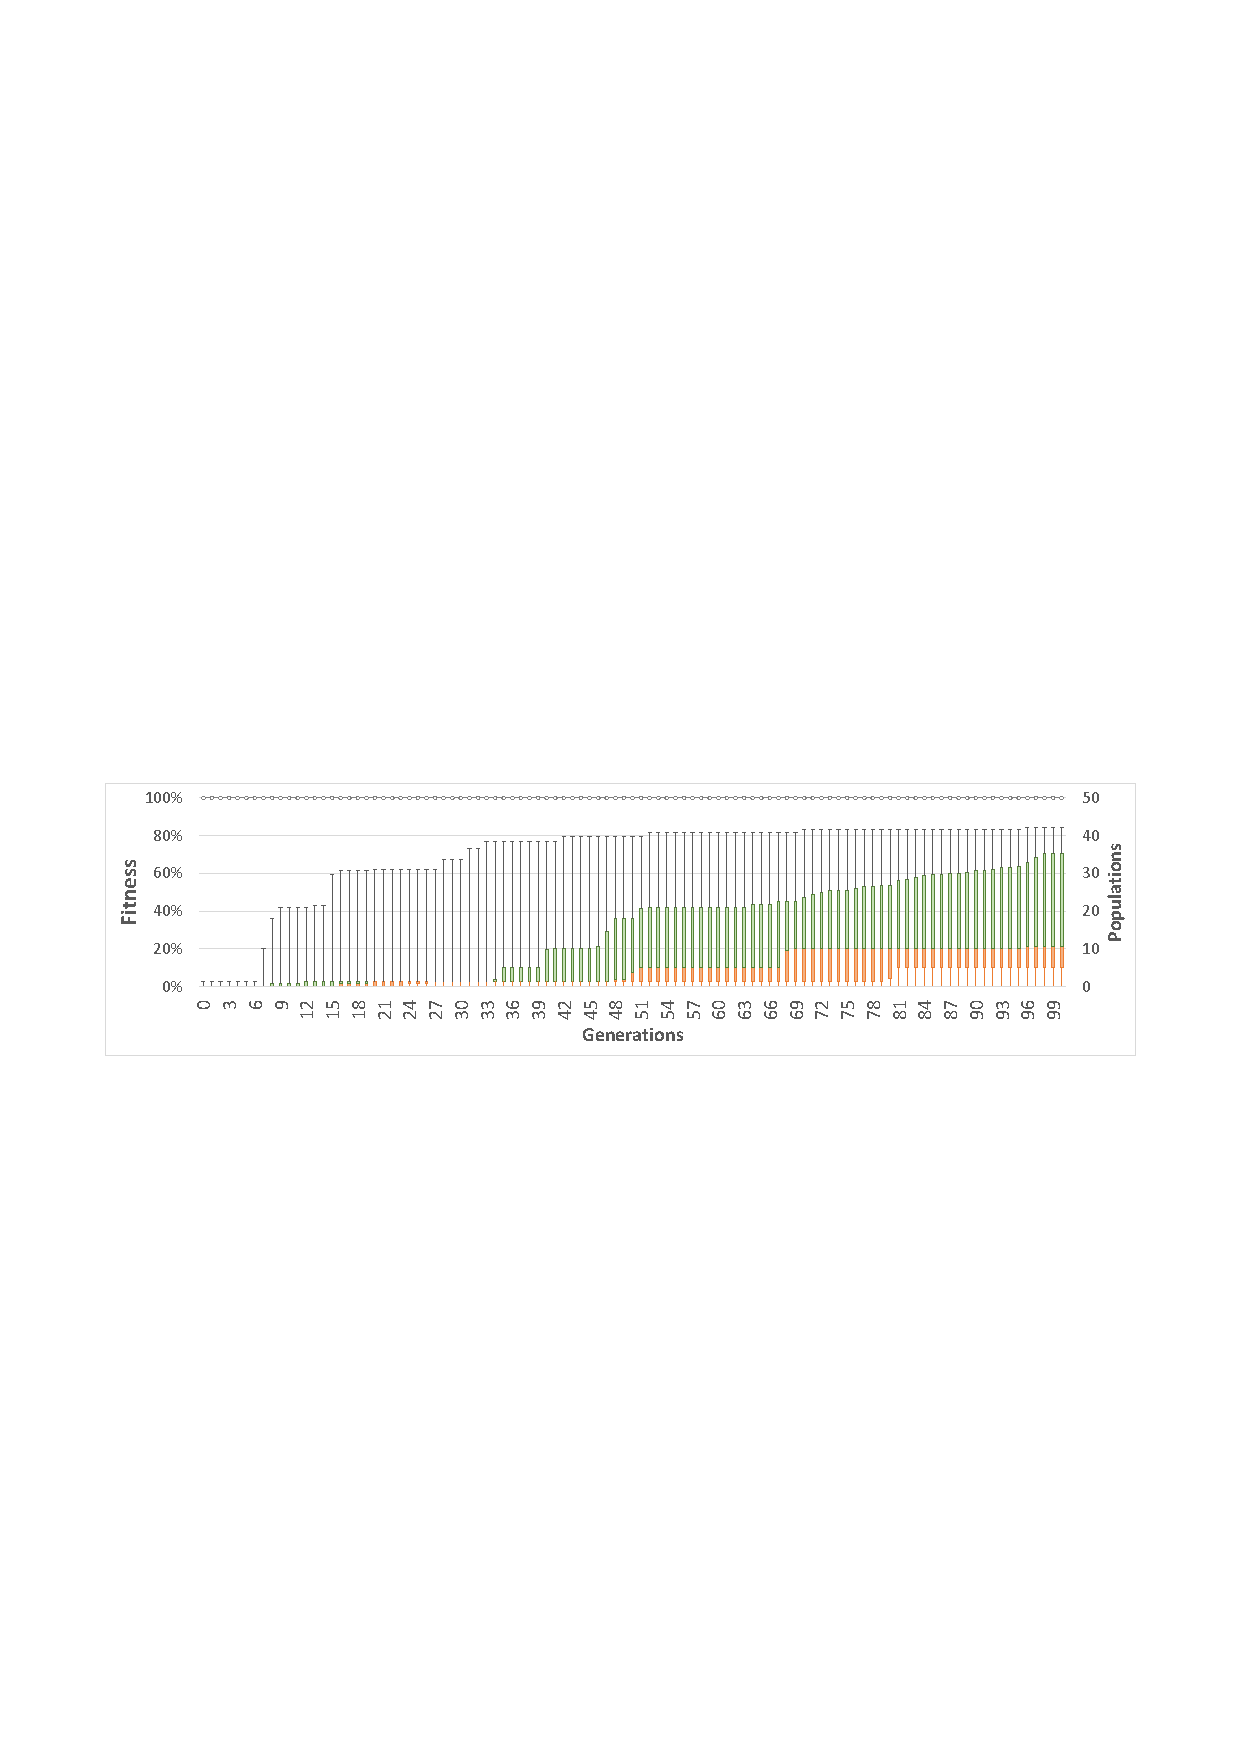
\includegraphics[scale=0.8, trim=1.5cm 11.5cm 1.5cm 13cm, clip=true]{Images/ConfigurationComparison_TournamentSize10.pdf} 
	\caption{Configuration development with ``Tournament selection with elitism - Tournament size of 10"-Selection and Replacement Strategy. All other settings are equal to the recommended configuration.}
	\label{figConfigurationComparison_TournamentSize10}
\end{figure}

The size of two instead of ten renders this strategy not that inertial, but it also results in the highest possible selection pressure within this strategy. Also, the ``Roulette wheel selection with elitism"-Strategy does not achieve the same performance as the naive one. The fitness rise of the maximum fitness is almost equal in the first \glspl{Generation} to the recommend configuration. Although the fitness median then stays at about 20\%, which is probably why the fitness maximum also does not increase with the same pace anymore.
 
\textbf{Fitness Function analysis}: Within the recommended configuration, the one using the heuristic comparison is included. Hence, at first the question is, how it compares to the one using the pure Name-based method. Figure \ref{figConfigurationComparison_BestWithBalancedFitnessFunction} shows the development of this ``Class focused using Name"-Fitness Function, with the major observation that the maximum fitness becomes stuck at about 85\%. A rough analysis of a few \glspl{Individual} showed that the``Name"-\glspl{Property}, which have to be transformed using the ``Merge Name Identity" pattern, blocked the algorithm. Since the ``Name" is a prerequisite for many further improvements within this \gls{FitnessFunction}, it is clearly outperformed by the heuristic comparison method.

\begin{figure}[!ht]
	\centering
	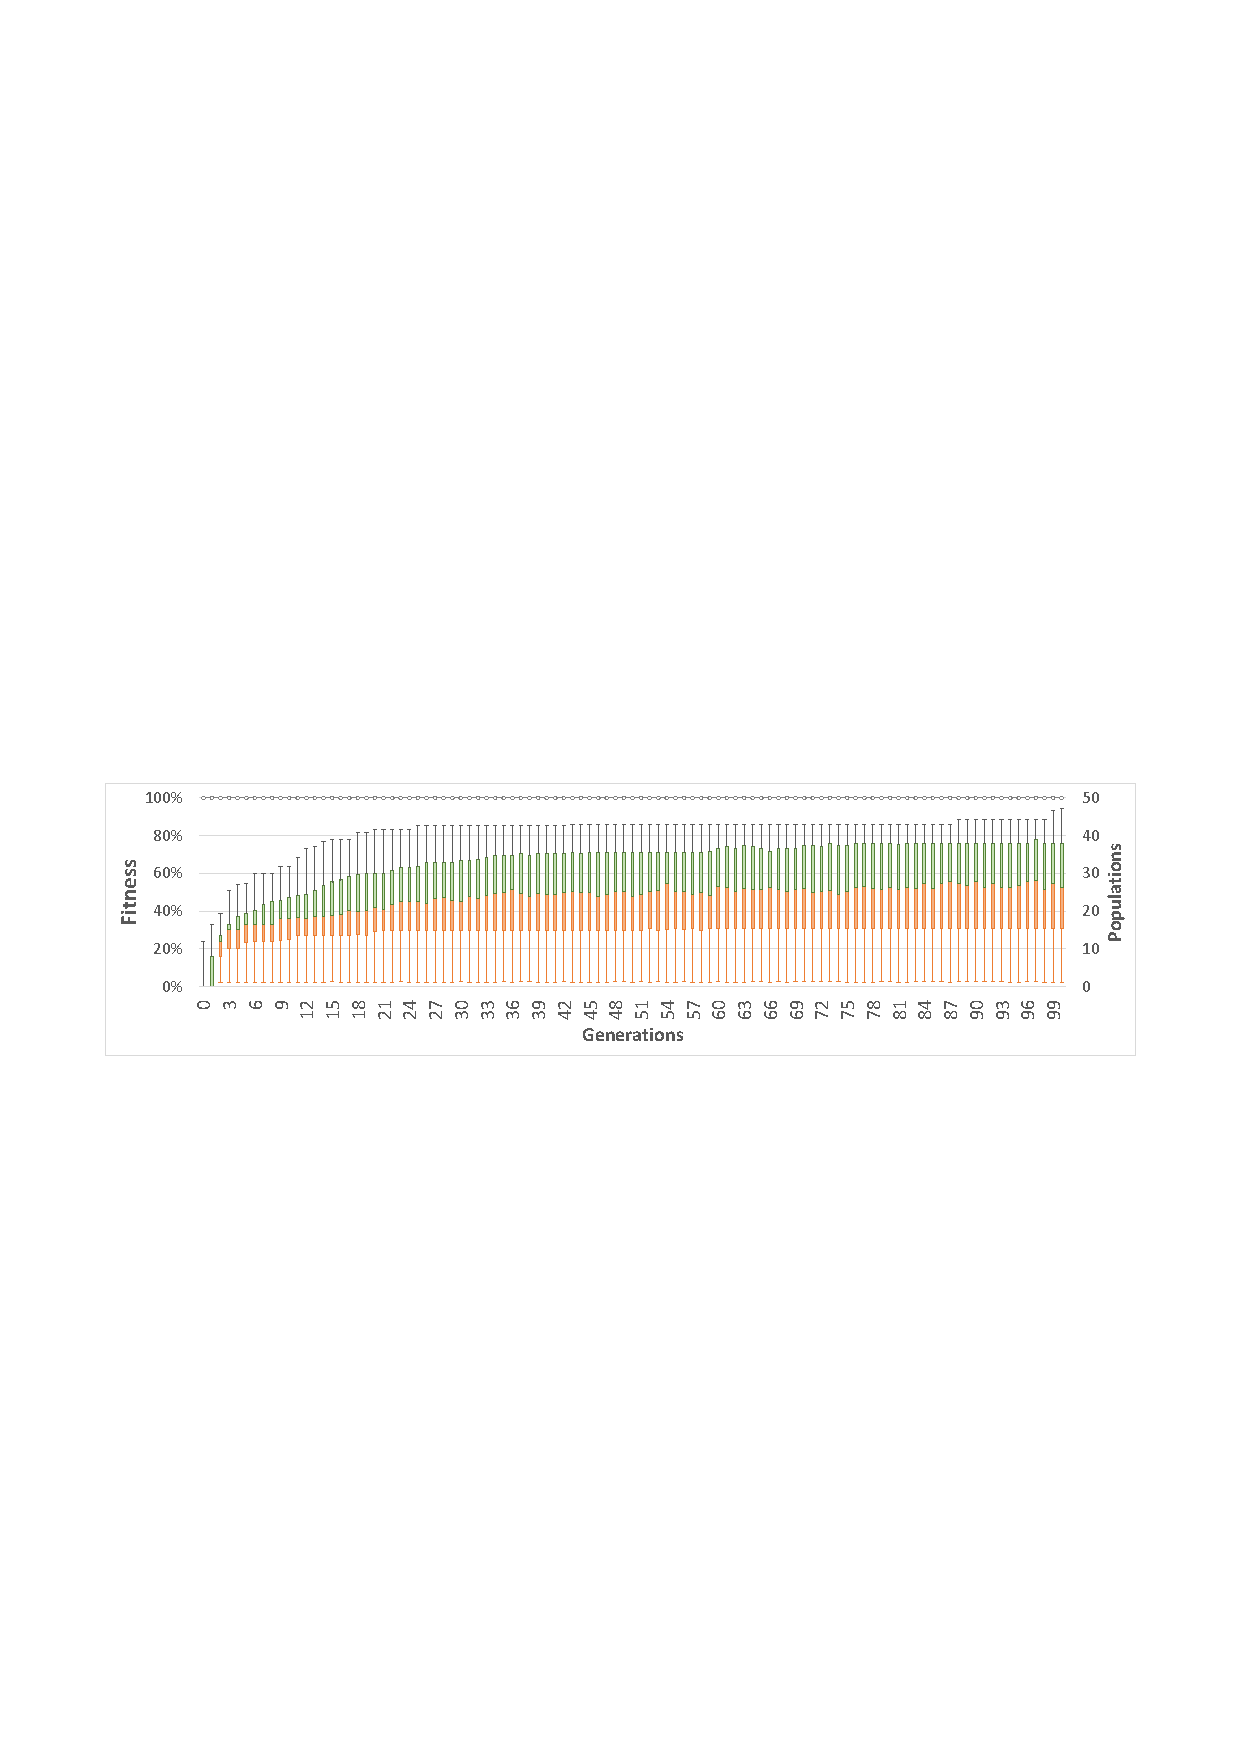
\includegraphics[scale=0.8, trim=1.5cm 11.5cm 1.5cm 13cm, clip=true]{Images/ConfigurationComparison_BestWithBalancedFitnessFunction.pdf} 
	\caption{Configuration development with ``Class focused using Name"-Fitness Function. All other settings are equal to the recommended configuration.}
	\label{figConfigurationComparison_BestWithBalancedFitnessFunction}
\end{figure}

The ``Class focused using Name and heuristic fall-back"-Fitness function which uses a combination of both was very close to the pure heuristic function. This slight difference is considered as insignificant.

All the other functions differed only through their weights and showed a similar behavior compared to the ones with the same comparison method. Thus, weights are not relevant in the two scenarios.

 
\textbf{Mutation Selection Strategy analysis}: Figure \ref{figConfigurationComparison_BestWithOption} shows the fitness development using the ``Option"-Mutation Selection Strategy. Within this strategy the major part of the \gls{Population} is especially at the beginning far below the ``Operator $\rightarrow$ Option"-Strategy. The maximum fitness increases in the further \glspl{Generation} only slowly. This is probably due to the fact that some \glspl{Mutation} have too many options that do not change the fitness. Too many options that decrease are less likely, since the fitness distribution is stable.

\begin{figure}[!ht]
	\centering
	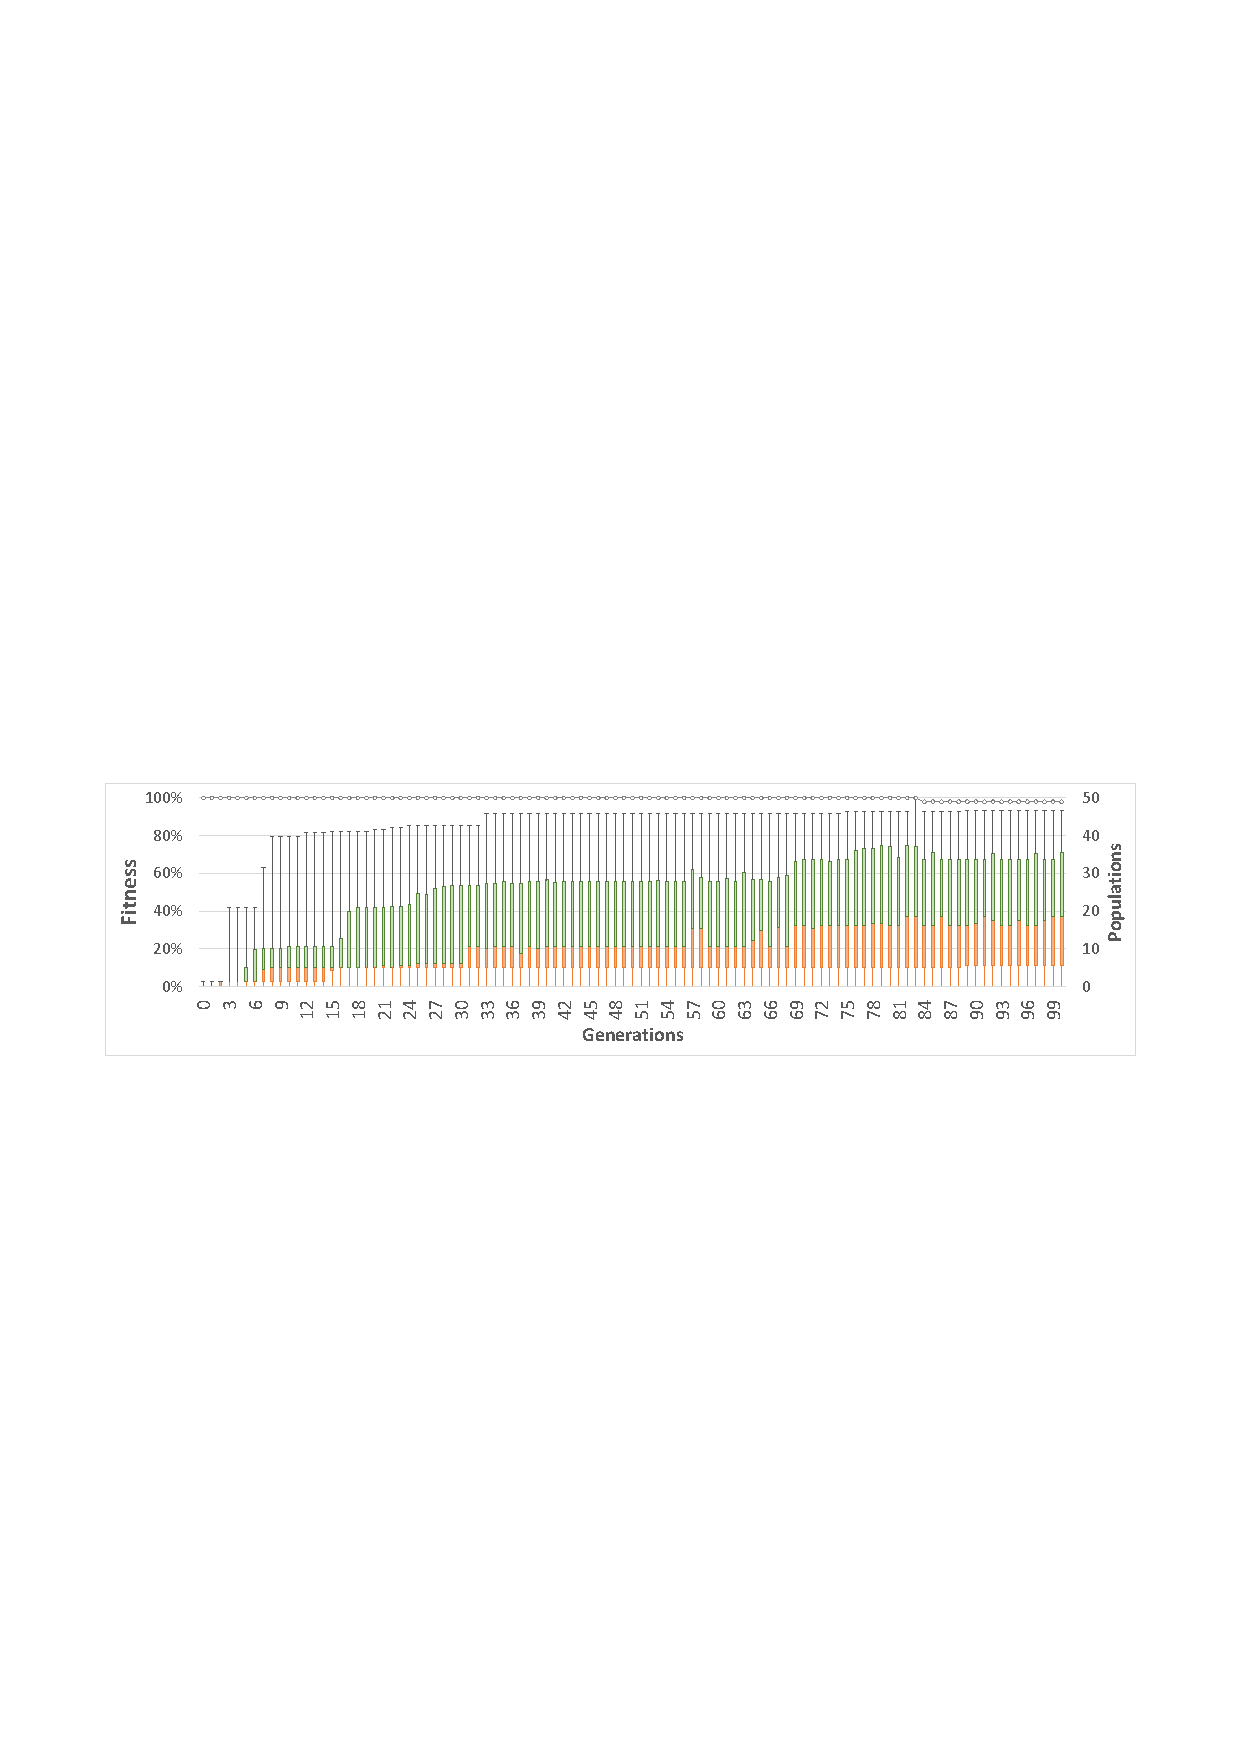
\includegraphics[scale=0.8, trim=1.5cm 11.5cm 1.5cm 13cm, clip=true]{Images/ConfigurationComparison_BestWithOption.pdf} 
	\caption{Fitness development of ``Option"-Mutation Operator Selection Strategy. All other settings are equal to the recommended configuration.}
	\label{figConfigurationComparison_BestWithOption}
\end{figure}

A rough analysis showed that i.e. the add-\glspl{Mutation} of ``One Object-to-Many Objects of same Type" and the related ``Merge Name Identity" pattern create hundreds and sometimes thousands of options, which all result in no fitness change. Hence, those are not distinguishable for the algorithm rendering it a random search. Selecting the ``Mutation" first provides a larger probability that options are chosen that create any change and therefore provide a better guidance for the algorithm. Especially in the first \gls{Generation} the ``One-to-One Object of same Type" pattern increases the fitness fast. 


\textbf{\Gls{Population} size and maximum number of \glspl{Generation} analysis}: As already explained in the previous section, an increase of these two settings increases the chance to identify a solution in the recommended configuration. A reduction reduces the execution time and required computational power, but a \Gls{Population} size below 10 does already in the simple example return often no solution. Executing the recommended configuration with a \gls{Population} size of 10 instead of 100, keeps the minimum, 25$^{th}$ percentile, median and the 75$^{th}$ Percentile at 0\% over all 100 \glspl{Generation}. The maximum ends at about 20\%. Hence at least 50 \glspl{Individual} are required by the algorithm in any case, otherwise a termination with a solution is almost impossible.

\section{Maintainability of Results}
\label{secMaintainabilityOfResults}

This section provides a rough assessment of the solutions using only a few metrics that were considered important in this context. Usually, software systems consist of a large number of \glspl{Class} and modules, whereas the created \glspl{ModelToModelTransformation} are small pieces of code. Thus, an application of the whole bandwidth of quality metrics is rendered useless.

Measuring the quality is focused on readability and comprehensibility of the created source code, whereas the former aids the latter \cite{Buse2008}. Furthermore, also the test-coverage is evaluated. Since \gls{ModelTransformationByExample} relies on examples, which are test cases according to the Test-Driven Development methodology \cite{Beck2002}. Hence, it is relevant to measure to which extended the created source code is actually used to solve the given examples. Other common quality metrics like efficiency are not applied, since the primary focus is that the solutions are adaptable by humans.

First an overview of the solutions is provided. In general, the created \glspl{ModelToModelTransformation} are similar or identical to the ones presented in listing \ref{lstETLSimpleExample} for the simple scenario and listing \ref{lstETLComplexExample} for the complex scenario. Overall, the evaluation created about 2.000 different solutions for the simple and about 200 for the complex scenario (see section \ref{secRecommendedConfiguration}). A review of random samples showed that the variations result to a large extend out of different \gls{TransformationRule} orders or statement orders. Furthermore, also semantically different solutions were created by using the potential of \glspl{Association}. Since they connect two \glspl{Property}, a transformation can start from both sides which also causes variations. Finally, for the complex scenario also solutions specifically targeted at the provided example pair were created that do not work in a common situation. 

\begin{figure}[!ht]
	\centering
	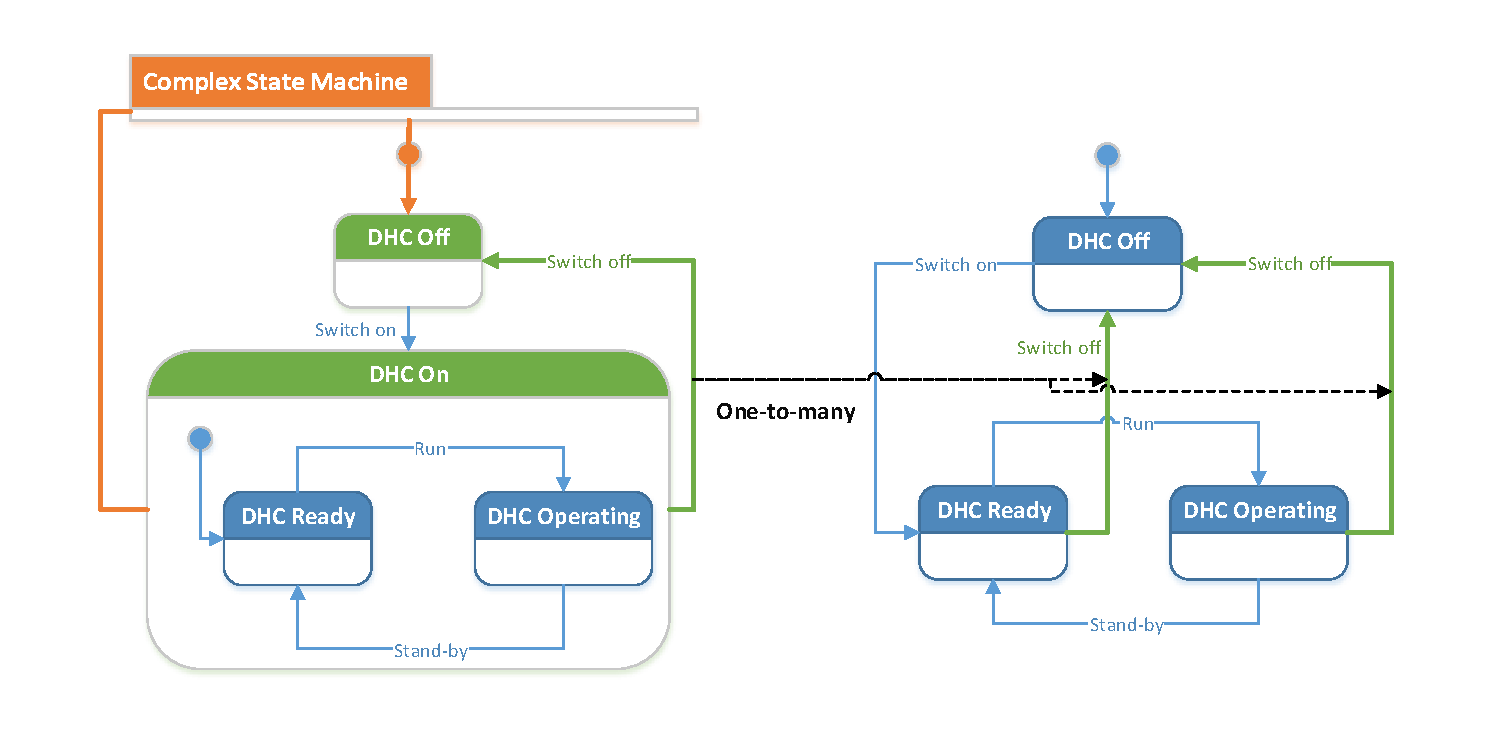
\includegraphics[scale=0.6, trim=0cm 1cm 0cm 0cm, clip=true]{Images/UnexpectedShortcut.pdf} 
	\caption{Transformation Pattern ``One Object-to-Many Objects of same Type" used in some cases the containment \glspl{Association} to the Complex State Machine instead of the Transition to query ``DHC Off"}
	\label{figUnexpectedShortcut}
\end{figure}

Figure \ref{figUnexpectedShortcut} shows such a situation. The Transformation Pattern ``One Object-to-Many Objects of same Type" used the containment \glspl{Association} to the Complex State Machine instead of the Transition-Target to query ``DHC Off". This solution is not the expected generic solution and works only within such a special case, since the Target of such a Transition is not always the Initial State of the Complex State Machine at the same time. It is not an error in the algorithm. Rather, the provided example was ambiguous and has to be refined. After presenting the range of solutions, the defined quality metrics are evaluated in the following.

\textbf{Test-Coverage}: The first criteria, source code coverage by unit tests, is achieved by removing unused \glspl{TransformationRule}. Since the examples represent the test cases, the code always has 100\% test coverage.

\textbf{Readability}: The judgment of readability is dependent on the reader, but \cite{Buse2008} identified low level metrics that on average capture the common understanding of readable source code. On behalf of those together with human annotations, \cite{Buse2008} trained a classifier which is able to measure the quality of source code. The tool and human annotations are targeted at the language Java and thus cannot be used to measure the quality. Therefore, the metrics of \cite{Buse2008} are used as a guideline. For a readability analysis the presented reference solutions are used, since the other solutions are variations with a similar appearance.

The top five criteria from \cite{Buse2008} that reduce the readability, are the average length of identifiers, the average line length, the average number of brackets, the maximum line length and the average indentation. The top two positive effects are the average number of blank lines and the average number of comments. 

The length of identifiers is long with up to 50 characters. Since the names of i.e. variables reflect the transformed type like ``complexStateMachine" in ``transform complexStateMachine : Source!ComplexStateMachine", they improve the readability from a subjective point of view compared to short forms like ``csm". Also rule names are sometimes even longer, i.e. ``TransitionFromComplexState To ManyTransitions", but also thereby provide a good explanation of its contents.

Due to the length of some identifiers, also some lines become long with about 150 characters. Especially, the context-sensitive \glspl{TransformationRule} require property chains like ``a.b.c" which also contribute to longer lines. Since the depth is limited to less than three \glspl{Property} (see subsection \ref{secClassTransformation}), this is barely acceptable.

The average number of brackets is very low and the lines of code encapsulated within blocks by brackets does not exceed ten lines. Also, the subjective impression renders the structure provided by those blocks well-arranged.

Indentation is used for the contents of a \gls{TransformationRule} and the contents of a loop. All other statements are assignments and do not result in any indentation. Hence, the indentation is usually one within a \gls{TransformationRule} and at least two within a loop, which is a rather low and thus a positive value.

Blank lines are used to separate \glspl{TransformationRule} and the header of a rule from the statements. This results in two blank lines per rule, thus overall six to ten are used in a solution compared to 20 to 60 lines of code. This proportion is considered as well-balanced from a subjective point of view.

The number of comments, which is the last considered criteria, is zero since those are not generated and hence have a negative impact on the quality from a general perspective. From a subjective one those are not required, since the \glspl{TransformationRule} contain descriptive names. Nevertheless, shorter rule names and comments which contain the detailed information might improve the readability. 

\textbf{Comprehensibility}: Rating the comprehensibility depends also on the reader. No general measurement has been found which is applicable and useful in the domain of \gls{ModelToModelTransformation}. Therefore, this analysis is to a certain extend subjective. 

% i.a. due to the good readability
Overall, the understandability of the created solutions is quite good. The names of \glspl{TransformationRule} and variables reflect the underlying semantic. For example a rule name has the form ``Source2Target", and hence enable the reader to quickly identify the general concept of the transformation. Also, the usage of patterns improves the comprehensibility, especially when those patterns are well known. Nevertheless, there are obstacles, which often render an overall quick understanding difficult. Some statements are redundant, e.g. an \gls{Association} is transformed on both ends, whereas one is sufficient. Sometimes also contradictory \gls{Association} transformations occur, where the latter \gls{Property} transformation overrides the former. This adds unnecessary complexity and is sometimes difficult to understand. Furthermore, using a different \gls{Association} end, may create solutions in a roundabout way, which is sometimes not intuitive. Additionally, unexpected solutions like the one presented in figure \ref{figUnexpectedShortcut} impede the legibility. Those use specifics of the example pair, which was not intended.

\textbf{Overall rating}: The maintainability is quite good in general due to the readable names, well-formed code structure and absence of unused code. However, the comprehensibility suffers in some solutions especially of the complex scenario, due to redundant or contradictory assignments and overcomplicated approaches.